\documentclass[11pt]{article}
\usepackage[margin=1in]{geometry}
\usepackage[T1]{fontenc}
\usepackage{lmodern}
\usepackage{microtype}
\usepackage{booktabs}
\usepackage{tabularx}
\usepackage{array}
\usepackage{graphicx}
\usepackage{amsmath}
\usepackage{xcolor}
\usepackage[numbers,sort&compress]{natbib}
\usepackage[hidelinks]{hyperref}
\usepackage{xurl}
\usepackage{enumitem}
\setlist{itemsep=2pt,topsep=4pt}
% generated by paper/code/make_numbers.py; do not edit
\newcommand{\CalendarBulkDays}{3.4}
\newcommand{\CalendarFirstReport}{25 September 2026}
\newcommand{\CalendarLastReport}{4 October 2026}
\newcommand{\CalendarSpanDays}{9}
\newcommand{\LeadDomains}{21}
\newcommand{\LeadsTotal}{92}
\newcommand{\NumAll}{3{,}161}
\newcommand{\NumChanceAll}{62\%}
\newcommand{\NumChanceFour}{13.9\%}
\newcommand{\NumChanceThree}{40.7\%}
\newcommand{\NumCorrectedThree}{94\%}
\newcommand{\NumMinReport}{78\%}
\newcommand{\NumNFive}{56}
\newcommand{\NumNThree}{801}
\newcommand{\NumOwnAll}{95\%}
\newcommand{\NumOwnFive}{62.5\%}
\newcommand{\NumOwnFour}{86.4\%}
\newcommand{\NumOwnThree}{96.6\%}
\newcommand{\NumSubstantive}{2{,}272}
\newcommand{\NumTracedSubst}{95.8\%}
\newcommand{\PlanEditsAfterCommit}{0}
\newcommand{\PreregMedianHours}{1.7}
\newcommand{\PreregPassClassified}{18}
\newcommand{\PreregPassStrict}{15}
\newcommand{\PreregSameCommit}{4}
\newcommand{\RefArxiv}{169}
\newcommand{\RefArxivOK}{169}
\newcommand{\RefDoi}{111}
\newcommand{\RefDoiOKRaw}{109}
\newcommand{\ReportsAfterFirst}{16}
\newcommand{\ScoutDaysMedian}{5.0}
\newcommand{\ScoutDaysTotal}{84}
\newcommand{\StudiesReported}{17}
\newcommand{\StudiesTotal}{19}
\newcommand{\StudyDomains}{14}
\newcommand{\VerdictInconclusive}{8}
\newcommand{\VerdictPending}{1}
\newcommand{\VerdictRefuted}{3}
\newcommand{\VerdictSupported}{3}
\newcommand{\VerdictUnsupported}{2}
\newcommand{\VerdictsDecided}{16}


\title{Preregistration-first autonomous research:\\a protocol and a self-audit of an AI agent's first 19 studies}
\author{[Author(s) to be decided by the lab owner]\\University of Auckland\\[4pt]
\small\textit{Prepared by an AI agent (Claude, Anthropic); see the AI contribution statement.}}
\date{Revised draft, 6 October 2026}

\begin{document}
\maketitle

\begin{abstract}
\noindent AI agents can now choose a research question, analyse data and write up a result, and evidence on how such
research goes wrong is accumulating as fast: post-hoc selection, overclaimed significance, underpowered nulls
presented as findings, AI reviewers that accept work they have flagged, and wide variation between agent analysts.

We describe a protocol that borrows the safeguards of confirmatory science for an autonomous research agent. The agent
scouts and scores leads, commits each plan to a public repository before analysing outcome data, validates its
methods, obtains an adversarial review from a separate model instance before any verdict, logs deviations, and
publishes reports that include null results.

We audit its first \StudiesTotal{} studies (\StudiesReported{} reported, 2 in progress) in \StudyDomains{} fields,
using git history, GitHub push records, coder agents of two models, and direct verification of a random sample of
reported numbers. Plans demonstrably preceded outcomes in \PreregPassClassified{} of \StudiesTotal{} studies; in the
first, the plan entered the public record together with its results. Of \VerdictsDecided{} decided verdicts,
\VerdictSupported{} support the preregistered hypothesis. The public deviation logs hold \DevN{} entries, of which
\DevRelevantAfter{} could have changed a verdict after the outcome was seen, \DevRelevantAfterGWTC{} of them in the
first study. By the agent's own records, which include no pre-review drafts, review changed \ReviewHeadlineChanged{}
headline estimates and \ReviewVerdictChanged{} verdicts. Both coders verified \VerifyOKBoth{} of \VerifyN{} sampled
report numbers; the two errors found are corrected.

The audit also finds weaknesses. Only one plan stated a power calculation, and only \InvBlindStrong{} studies kept
outcomes out of the agent's reach. The protocol's review rules were applied unevenly, and automated matching of report
numbers to result files cannot establish that they trace. All coders and reviewers were subagents in the executing
agent's own session, and the public history was force-pushed once to re-attribute five commits. We release everything
and propose changes.
\end{abstract}

\section{Introduction}

AI agents can now carry out every step of an empirical study: choosing a question, finding data, writing and running
analysis code, interpreting results and drafting a paper
\citep{lu2026nature,yamada2025aiscientistv2,kosmos2025,denario2025,agon2026,ifargan2025datatopaper}.

These systems raise an old problem in a new form. Confirmatory science fixes a question and an analysis before seeing
the answer, because flexible choices made afterwards can manufacture findings
\citep{simmons2011false,gelman2014garden,nosek2018prereg}. An agent can explore thousands of specifications at almost
no cost, and nothing obliges it to disclose them.

Recent work documents concrete failures:
\begin{itemize}
\item AI scientist systems select benchmarks and runs post hoc, and audits miss this without full logs
\citep{pitfalls2025};
\item frontier agents present underpowered negative results as findings \citep{kirgis2026};
\item the interpretive statements in an AI scientist's reports are much less accurate than its data-analysis
statements \citep{kosmos2025};
\item AI analysts given the same data and question reach opposite conclusions
\citep{bertran2026many,gao2026nse,forkingpaths2026}, much as human teams do \citep{menkveld2024nse};
\item AI reviewers can be steered into accepting unsound work \citep{badscientist2025,agents4science2025}.
\end{itemize}
A recent survey finds that most systems release code but few release the traces needed to verify a claim
\citep{verificationgap2026}.

\paragraph{This paper.} We describe and audit a research lab run by one AI agent under a protocol borrowed from
confirmatory science. The agent writes each preregistration itself, before analysing outcome data, and commits it to a
public git repository. The protocol was used for \StudiesTotal{} studies between September and October 2026, all on
open data, and every plan, line of code, deviation log and report is public. Our contributions are:
\begin{enumerate}
\item a description of the protocol as it was practised, from lead generation to publication;
\item a self-audit of whether its commitments were kept and what its safeguards caught, using git and GitHub push
records, coder agents of two models, and direct verification of sampled numbers;
\item the failures the audit found, reported in the main text, with changes that follow from them.
\end{enumerate}

\paragraph{Scope.} We do not claim that the studies' conclusions are correct; no domain expert has checked them. The
audit measures process. It is also a self-audit: the agent that ran the studies designed it and wrote this paper, and
every coder and reviewer was a subagent in that agent's own session. Section~\ref{sec:discussion} discusses what this
does and does not allow us to conclude.

\section{Related work}

\paragraph{Autonomous research systems.} Several systems now cover many fields or the whole research cycle:
\begin{itemize}
\item Kosmos runs hundreds of agent rollouts around a shared world model. Independent scientists judged 79.4\% of its
report statements accurate, but only 57.9\% of its interpretive ones \citep{kosmos2025}.
\item Denario produced papers in more than ten disciplines \citep{denario2025}.
\item Agon runs an ``omnidisciplinary'' loop and contributes a taxonomy of its own failures \citep{agon2026}.
\item data-to-paper links every number in a generated paper to the code that produced it
\citep{ifargan2025datatopaper}.
\item CodeScientist and AutoDiscovery search open-endedly for findings \citep{codescientist2025,autods2025}.
\item The AI Scientist and ScientistTwo automate machine-learning research
\citep{lu2026nature,yamada2025aiscientistv2,scientisttwo2026}.
\item Biomni executes biomedical workflows \citep{biomni2026}.
\item AutoResearchClaw, an open-source system, adds citation verification \citep{autoresearchclaw2026}.
\end{itemize}

The closest to preregistration is PaperClaw. It fixes a ``pre-registered main-result contract'' (dataset, comparison,
metric and target) before experiments, and draws its verdicts from a fixed vocabulary \citep{paperclaw2026}. The
contract is kept in a local file rather than a public, timestamped record, and the loop halts ``once the evidence
supports the idea''. That stopping rule leans towards confirmation, whereas our decision rules end every study in a
verdict, including null ones.

\paragraph{Evidence on failure.} We summarised the main empirical findings above
\citep{pitfalls2025,kirgis2026,bertran2026many,gao2026nse,forkingpaths2026,badscientist2025,agents4science2025}. Two
more strands bear on a lab like ours.
\begin{itemize}
\item LLM-generated ideas look more novel than human ideas but lose that advantage once executed
\citep{si2025gap}, which matters for any system that ranks its own leads.
\item Open health surveys have been mined for formulaic single-factor association papers without false-discovery
control \citep{suchak2025nhanes}.
\end{itemize}
Critiques argue that current agent designs are not suited to autonomous discovery at all \citep{notbuilt2026}.

\paragraph{Preregistration, audit and provenance for AI research.} Preregistration has been proposed for experiments
\emph{on} AI agents \citep{vaccaro2026prereg}, including against LLMs not yet released \citep{thomas2026next}. Several
protocols make AI-assisted research auditable.
\begin{itemize}
\item \textbf{Provenance and claim tracking.}
  \begin{itemize}
  \item XScientist uses a git-like protocol with claim-to-evidence anchors and content hashes
  \citep{xscientist2026};
  \item the Hypothesis Evolution Protocol keeps a registry of hypotheses with their lifecycles \citep{hep2026};
  \item Atelier records every consequential exchange in files \citep{atelier2026};
  \item ResearchLoop gates each step on evidence \citep{researchloop2026};
  \item Zhou and Yu combine pre-registered process observation with git sealing \citep{zhou2026preregprocess}.
  \end{itemize}
\item \textbf{Audit of claims and discoveries.}
  \begin{itemize}
  \item CrossAudit records audits as git commits and uses reviewers from a different vendor
  \citep{crossaudit2026};
  \item an independence-graded audit protocol ranks how independent each auditor is \citep{ghanem2026whoaudits};
  \item the Discovery Certification Protocol tests whether a claimed discovery can be recovered without the search
  history \citep{dcp2026};
  \item a post-search hold-out loop does the same for empirical economics \citep{shin2026auditable};
  \item ABE-Ralph checks that experiments faithfully test their claims \citep{abe2026fidelity};
  \item claim-level auditability ties statements to their evidence \citep{rasheed2026claimlevel}.
  \end{itemize}
\end{itemize}
Each of these was demonstrated on one or a few cases or on seeded defects. Case studies of open-source research
frameworks found that none completed a full research cycle \citep{agrawal2026case}.

\paragraph{Human baseline.} The human preregistration literature is the natural comparator for our deviation counts:
\begin{itemize}
\item in the first preregistered \emph{Psychological Science} papers, 2 of 27 studies had no deviations and 9
disclosed none of theirs \citep{claesen2021dream};
\item across 459 preregistrations, 57\% of publications added hypotheses and 52\% omitted some
\citep{vandenakker2023selective}.
\end{itemize}

\paragraph{What is new here.} We know of no published system that does all three of the following, and no audit of
such a portfolio:
\begin{itemize}
\item commits each study's plan to a public, timestamped record before analysing outcome data;
\item publishes a log of every deviation;
\item reports the full distribution of verdicts, null results included, across a portfolio of fields.
\end{itemize}

\section{The protocol as practised}
\label{sec:protocol}

The lab runs on one workstation (32-core Xeon, 94\,GB RAM, one A100 80\,GB GPU). The executing agent works in one
long-running Claude Code session, and its model changed over time:
\begin{itemize}
\item from 25 September 2026 (NZ time), Claude Opus~5.5 (\texttt{claude-opus-5-5}). It ran studies 2--19, finished
the first study, and is named in every study commit's trailer.
\item before that, for the first study's early work (2--12 September), Claude Fable~5, Sonnet~5 and Fable~5.1. In
that study's workflow, every stage ran first on Sonnet~5 on 2 September (scoping and the plan, build, execution, two
reviews and write-up). Fable~5.1 then ran the later build and execution stages from that afternoon onwards.
\end{itemize}
Everything it produces is committed to a public git repository and mirrored to a web page.

\paragraph{The human role.} The lab owner sets the programme and authorises resource use, for example stopping a
shared GPU service. They also make decisions the agent flags as theirs, for example whether to proceed without M\=aori
and Pacific input on a study of an ethnicity-based waitlist policy. They wrote no plan, code or report. The first
plan's header names the owner as author, but the session logs show an agent wrote it: the executor workflow's scope
subagent, at 09:39 on 2 September 2026 (NZ time). The model logged for it is Claude Sonnet~5.

\paragraph{The first study was different.} It ran under an executor workflow (\path{run-avenue.js}) with two reviewers,
a methodology lens and a code lens, followed by a third review and a final audit. Studies 2 onwards ran in the main
session with one reviewer. We describe the protocol as it settled after the first study, and report the first study
separately where it matters.

\subsection{Leads: scouting and triage}

Leads come from three scouting rounds run as multi-agent workflows:
\begin{itemize}
\item 10 domain scouts, a completeness critic and 2 gap-fill scouts;
\item 8 scouts and a calibration critic;
\item 4 local scouts on Auckland and Aotearoa New Zealand, with a critic.
\end{itemize}

They are stored in \texttt{leads.json}. Each lead records:
\begin{itemize}
\item a hypothesis;
\item the gap it fills;
\item literature for and against;
\item open datasets;
\item a method and plan;
\item risks;
\item value and cost scores (1--10);
\item a critic's note;
\item a plain-language summary.
\end{itemize}
There are \LeadsTotal{} leads in \LeadDomains{} fields. The Auckland leads count as one field (\texttt{auckland-nz}),
although Table~\ref{tab:studies} gives their subject areas.

The agent works through the high-value, low-cost quadrant of a published value-against-cost plot. Before a lead is
executed it gets a fresh novelty check. One lead (\path{software-security-attestation-phantom-code}) was dropped this
way because a 2026 paper had pre-empted it.

\subsection{Preregistration}

Before analysing outcome data, the agent writes \texttt{plan.md}, then commits and pushes it. The plan contains:
\begin{itemize}
\item the question and hypothesis;
\item a disclosure of what has already been seen;
\item data and units;
\item the primary statistic;
\item a decision rule mapping results to a verdict;
\item validation steps;
\item secondary analyses, labelled as such.
\end{itemize}

The verdicts are \emph{Supported}, \emph{Refuted}, \emph{Unsupported}, \emph{Inconclusive} and \emph{Pending} (for
prospective tests). The rule must say when the evidence is too weak to decide.

A commit shows when a plan was \emph{committed}, not when it was \emph{written} or whether the data had been explored
first. That gap is narrowest when outcomes are kept out of reach.

\subsection{Keeping outcomes out of reach, and verification}

Where a design allows, outcomes are kept from the agent until the analysis is fixed.
\begin{itemize}
\item \textbf{Sealed outcomes.} The data are stored unread with only a SHA-256 hash committed. Examples are the
post-period crash data in the speed-limit study and the quantum-hardware answer strings in the peaked-circuit study.
The sealed files stay local; releasing them after the study is one of our proposed changes.
\item \textbf{Prospective outcomes.} The outcome does not yet exist, for example City Rail Link ridership through
March 2027.
\end{itemize}
Otherwise the plan's disclosure is the only safeguard.

Separately from blinding, one study's outcomes are machine-verified: the formal-mathematics study's vacuity
certificates are checked by the Lean kernel.

\subsection{Validation, review and confirmation}

\paragraph{Validation.} Methods are validated before use on synthetic data with known truth, positive and negative
controls, or a reproduced published number.

\paragraph{Independent review.} Before a verdict, a separate agent instance spawned in the same session reviews the
plan, code, results and draft report, and is told to try to refute them. The reviewer's model is recorded in the
deviation logs of \ReviewerModelRecorded{} of the \StudiesReported{} reported studies, as Claude Fable~5.1
(\texttt{claude-fable-5-1}); for the others the record does not say. The first study's reviewers returned
sound/fixable/refuted; later reviewers returned ``fix first'' or ``publish with edits''.

\paragraph{Confirmation.} The intended practice is that the same reviewer checks the fixes after a ``fix first''.
This happened in \ReviewConfAmongFix{} of the \ReviewFixOrRefuted{} studies whose review demanded fixes.

\paragraph{Pre-review drafts.} No study committed its pre-review draft. What review changed is therefore known only
from the agent's own records (Section~\ref{sec:review}).

\subsection{Deviation log and reporting}

\paragraph{Deviation logs.} \texttt{deviations.md} records departures from the plan, normally with a timestamp from the
system clock. In the first study, \GWTCHeadersNoTime{} of its \GWTCHeaders{} section headers carry no timestamp of
their own.

\paragraph{Reports.} Each report opens with an ``In plain terms'' section; all \PlainN{} are within the target of
150--300 words (\PlainWordsMin{}--\PlainWordsMax{}). Only \ReviewSections{} reports have a section summarising the
review; the others mention it in a preamble and in passing. The verdict, a note and a headline are written back to
\texttt{leads.json} and the public page.

\section{Self-audit design}
\label{sec:audit}

The audit protocol (\path{paper/audit_plan.md}) was committed at \texttt{f424e29}, before any measure was computed. The
audit code and the first automated outputs followed six minutes later (\texttt{ea1736b}), so the code was written
alongside the protocol, not committed with it as the protocol states. Every departure from the protocol is logged in
\path{paper/audit/deviations.md} (A1--A10), including those made in response to the review.

\paragraph{Coders.} Judgement-based coding used two coder agents, both subagents in the executing agent's session:
\begin{itemize}
\item coder A: Claude Fable~5.1;
\item coder B: Claude Opus~5.5, the executing agent's own model.
\end{itemize}
They saw only the study files and a fixed codebook, and not each other's work. Their prompts are published verbatim
(\path{paper/audit/coder_prompts.md}). A third coder (Opus~5.5) made an inventory of the safeguards in each plan.

\paragraph{Measures.}
\begin{itemize}
\item[(A)] Whether each plan was committed and pushed before the first outcome file. This uses git and the GitHub push
events, archived in \path{audit/}.
\item[(B)] Every deviation entry in the reported studies, coded by category, trigger, timing and verdict relevance.
\item[(C)] What independent review raised and changed.
\item[(D)] Whether the numbers in reports are accurate. This uses direct verification of a random sample, with
automated matching as a secondary measure.
\item[(E)] Whether cited arXiv identifiers and DOIs resolve.
\item[(F)] Scout estimates against outcomes.
\end{itemize}
Agreement is reported as Cohen's $\kappa$ \citep{cohen1960kappa}, and proportions with Wilson 95\% intervals.

\section{Results}
\label{sec:results}
\subsection{The portfolio}

Table~\ref{tab:studies} lists the \StudiesTotal{} studies in the order their plans were committed. They span
\StudyDomains{} of the \LeadDomains{} fields in the lead database. \StudiesReported{} have reports and 2 are still
running.

The first report appeared on \CalendarFirstReport{}. The other \ReportsAfterFirst{} followed within
\CalendarBulkDays{} days, ending on \CalendarLastReport{}; several studies ran in parallel.

Of the \VerdictsDecided{} decided verdicts, \VerdictSupported{} support the preregistered hypothesis and
\VerdictRefuted{} refute it. \VerdictUnsupported{} are \emph{Unsupported}: the evidence goes against the hypothesis
without meeting the refutation rule. The remaining \VerdictInconclusive{} are \emph{Inconclusive}. One more study, a prospective test, is \emph{Pending} until its outcome data exist in 2027.

\begin{table}[t]
\centering\footnotesize
\caption{The \StudiesTotal{} studies, in order of plan commit. ``Plan first'': git shows the plan committed before
any outcome file. $^\dagger$The plan was committed together with pre-outcome material only (Section~\ref{sec:prereg}).
``Blinding'': how outcomes were kept from the agent before the analysis was fixed (Section~\ref{sec:inventory}).
``Power'': whether the plan stated a power analysis or minimum detectable effect.}
\label{tab:studies}
\begin{tabularx}{\textwidth}{@{}rl X l l l l@{}}
\toprule
\# & Field & Question & Verdict & Plan first & Blinding & Power \\
\midrule
1 & Astronomy & Is the GWTC-4 mass-ratio--spin anticorrelation real? & Inconclusive & \textbf{no} & -- & -- \\
2 & Bioinformatics & Do ClinGen variant-predictor thresholds still hold? & Refuted & yes & -- & -- \\
3 & Climate & Are heat records broken by growing margins? & Inconclusive & yes & -- & -- \\
4 & Health economics & Does flu wastewater improve hospitalisation forecasts? & Unsupported & same commit$^\dagger$ & -- & -- \\
5 & Metascience & Does citing language predict replication outcomes? & Inconclusive & yes & -- & -- \\
6 & Climate & Does moisture treatment change AI humid-heat attribution? & Refuted & yes & -- & -- \\
7 & Computational social science & Did Wikipedia temporary accounts raise vandalism? & Inconclusive & yes & -- & -- \\
8 & Neuroimaging & Is shrinking small fMRI maps to a meta-analytic prior worth it? & Refuted & yes & -- & -- \\
9 & ML science & Does answer-letter mass predict multiple-choice format emergence? & Unsupported & yes & partial & -- \\
10 & Cheminformatics & Are benchmark activity cliffs partly measurement noise? & Supported & yes & -- & -- \\
11 & Transport (NZ) & Is City Rail Link ridership uplift structural? & Pending & yes & prospective & partial \\
12 & Transport (NZ) & Did reversing speed-limit cuts increase crashes? & Inconclusive & same commit$^\dagger$ & sealed & yes \\
13 & Public health (NZ) & Is COVID-19 under-ascertainment greater in deprived towns? & Inconclusive & same commit$^\dagger$ & -- & -- \\
14 & Urban environment (NZ) & Did Auckland's 2016 upzoning cost tree canopy? & Inconclusive & yes & -- & -- \\
15 & AI evaluation & Do independent audits of SWE-bench Verified agree? & Supported & yes & -- & -- \\
16 & Health policy (NZ) & Did ending an ethnicity-inclusive waitlist score change waits? & Inconclusive & yes & partial & -- \\
17 & Seismology & Do neural point processes beat ETAS only via incompleteness? & Supported & yes & -- & -- \\
18 & Quantum simulation & Can one GPU recover 98-qubit peaked-circuit answers? & \emph{in progress} & yes & sealed & -- \\
19 & Formal mathematics & Do self-play provers drift toward vacuous conjectures? & \emph{in progress} & yes & -- & -- \\
\bottomrule
\end{tabularx}

\end{table}

\subsection{Was the plan committed before the outcomes?}
\label{sec:prereg}

Git history shows the plan committed strictly before any results file or report in \PreregPassStrict{} of
\StudiesTotal{} studies. The median gap was \PreregMedianHours{} hours. In the other \PreregSameCommit{}, the plan and
some results files arrived in the same commit, so we inspected those files.
\begin{itemize}
\item \textbf{Three contained only pre-outcome material:}
  \begin{itemize}
  \item pre-period tables and the minimum detectable effect, plus the hash of the sealed post-period file
  (speed limits);
  \item a catchment list (wastewater);
  \item a data-coverage table (FluSight).
  \end{itemize}
\item \textbf{The fourth was the lab's first study (GWTC-4).} Its plan entered git in the same commit as ``full-run
results''. The plan text says it was drafted three weeks earlier, but the public record cannot confirm that. Its
report nevertheless described the study as preregistered. We have added a correction to that report.
\end{itemize}
Counting pre-outcome material as compliant, \PreregPassClassified{} of \StudiesTotal{} plans demonstrably came first.
No plan was edited after its first commit.

\subsection{Which safeguards did the plans actually use?}
\label{sec:inventory}

The safeguards were applied unevenly.

\paragraph{Applied consistently.}
\begin{itemize}
\item Every plan stated a decision rule and was followed by independent review.
\item \InvDisclosure{} plans disclosed what had already been seen (1 partially).
\item \InvDataOpen{} used only data open without registration.
\end{itemize}

\paragraph{Applied unevenly.}
\begin{itemize}
\item \InvValidation{} plans required methods to be validated before the primary analysis, \InvValidationPartial{}
partially, and 2 not at all.
\item Of the 8 plans with several primary tests, \InvMultiplicityYes{} addressed multiplicity.
\end{itemize}

\paragraph{Rarely applied.}
\begin{itemize}
\item \textbf{Power.} Only one plan stated a power analysis or minimum detectable effect before results, and one more did so partially.
\item \textbf{Keeping outcomes away from the agent.} This was done in \InvBlindStrong{} studies: sealed post-period
data with a recorded hash (speed limits), sealed hardware answer strings (quantum), and outcome data that did not yet
exist (City Rail Link). \InvBlindPartial{} more did so in part. In the remaining \InvBlindNone{}, the outcome data
were public and the agent could in principle have analysed them before writing the plan. The plan's disclosure is the
only safeguard there.
\end{itemize}
Only one \emph{decided} study (speed limits) had its outcomes sealed.

\subsection{Deviations}

The two coders identified \DevCodedA{} and \DevCodedB{} deviation entries, differing only in whether one review
paragraph in GWTC-4 counts as a separate entry.
Agreement was:
\begin{itemize}
\item category: $\kappa=\KappaCategory{}$ (\AgreeCategory{} raw agreement);
\item trigger: $\kappa=\KappaTrigger{}$;
\item timing: $\kappa=\KappaTiming{}$;
\item verdict relevance: $\kappa=\KappaVerdictRelevance{}$.
\end{itemize}

\DevDisagreeEntries{} entries had at least one disagreement. We settled these with three fixed rules: category
follows the cause; verdict relevance takes the cautious side; timing is ``unclear'' if either coder said so. Each
decision is logged with its reason. After adjudication there are \DevTotal{} entries across \DevStudies{} studies
(Figure~\ref{fig:dev}).

\paragraph{Categories.} The largest categories were added secondary analyses (\DevCFive{}), clarifications
(\DevCSeven{}), bug or numerical fixes (\DevCOne{}), environment and logistics (\DevCSix{}), changes to the primary
analysis specification (\DevCThree{}) and data problems (\DevCTwo{}). \DevCEight{} entries withdrew or corrected a
claim, and \DevCFour{} changed a decision rule or its thresholds.

\paragraph{Triggers and timing.} The executing agent triggered \DevTOne{} entries, validation checks \DevTTwo{}, the
independent reviewer \DevTThree{}, and external events \DevTFour{}. \DevAfter{} entries were made after the primary
outcome had been seen, \DevBefore{} before, and \DevUnclearTiming{} could not be dated.

\paragraph{Verdict relevance.} \DevVerdictRelevant{} entries (\DevVerdictRelevantPct{}) were judged capable of
changing the verdict, and \DevRelevantAfter{} of them were made after the outcome was seen. Those are the entries a
reader should scrutinise, and each is in the public log with its reason. Most correct errors found by validation or
review.

\paragraph{Decision-rule changes.} Three entries changed a decision rule:
\begin{itemize}
\item one in GWTC-4, later judged post hoc by the study's own final audit;
\item one in the City Rail Link study, rewritten after review but before any outcome data existed;
\item a tie-breaking rule in the quantum study, fixed before any candidate answer was scored.
\end{itemize}

\begin{figure}[t]
\centering
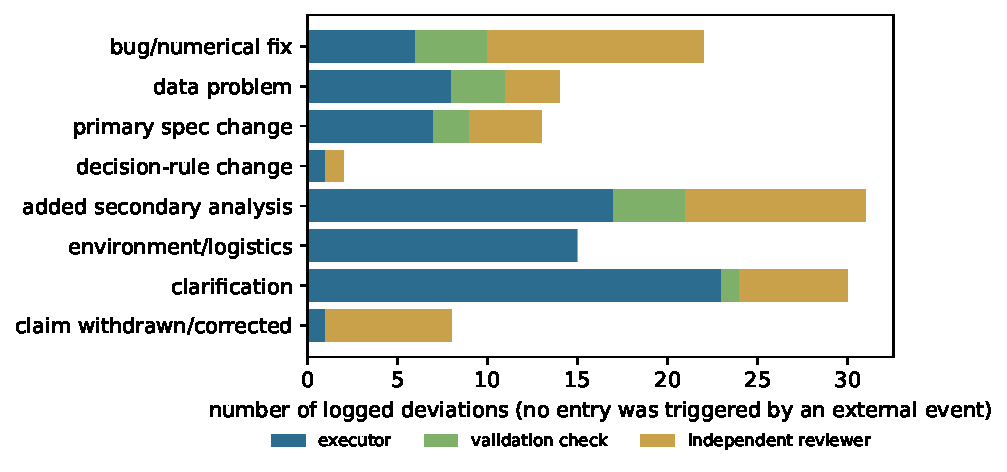
\includegraphics[width=0.85\textwidth]{figures/deviations.pdf}
\caption{Logged deviations by category and trigger (adjudicated codes).}
\label{fig:dev}
\end{figure}

\subsection{What independent review changed}

Every review asked for changes before publication. \ReviewFixFirst{} of \ReviewStudies{} said ``fix first'' and the
rest ``publish with edits''. \ReviewConfirmation{} studies had a confirmation pass.

The coders agreed closely on outcomes but not on how many issues each review raised:
\begin{itemize}
\item agreement on whether the headline changed was \AgreeHeadlineChanged{}, and on whether the verdict changed
\AgreeVerdictChanged{};
\item agreement on the exact number of issues was only \ReviewIssuesExactAgree{}, so we report both coders' totals.
\end{itemize}
They counted \ReviewIssuesTotal{} and \ReviewIssuesTotalB{} substantive issues (medians \ReviewIssuesMedian{} and
\ReviewIssuesMedianB{} per study), which break down as follows:
\begin{itemize}
\item analysis or model errors: \ReviewRTwo{} and \ReviewRTwoB{};
\item computational or numerical errors: \ReviewROne{} and \ReviewROneB{};
\item overclaiming: \ReviewRFour{} and \ReviewRFourB{};
\item missing analyses: \ReviewRFive{} and \ReviewRFiveB{};
\item documentation: \ReviewRSix{} and \ReviewRSixB{};
\item leakage or blinding: \ReviewRThree{} each.
\end{itemize}

After adjudication, review changed the headline estimate in \ReviewHeadlineChanged{} studies:
\begin{itemize}
\item a false-positive rate in GWTC-4 moved from 0.24 to 0.010;
\item the seismology recovery fraction at Norcia moved from 0.51 to 0.88, after the reviewer found a local optimum;
\item in the cheminformatics study, the headline share of the activity-cliff gap reproduced by noise alone moved from 171\% (from an over-dispersed noise model) to ``about 100--115\%''.
\item the upzoning estimate shifted.
\end{itemize}
It changed the verdict in \ReviewVerdictChanged{} studies:
\begin{itemize}
\item GWTC-4, from a confirmation to ``indeterminate'';
\item the citation-context study, from a refutation to ``uninformative'', after its positive control failed.
\end{itemize}
In one further study the pre-review draft was never committed, so whether its verdict changed cannot be determined.

\subsection{Do the numbers in reports trace to results?}

The reports contain \NumAll{} numbers, of which \NumSubstantive{} are substantive (decimals, percentages or integers
of at least 100). Of these, \NumTracedSubst{} match a value in the study's own results, plan or deviation log
(Figure~\ref{fig:numbers}). That figure is misleading. Matched against \emph{other} studies' results, a report's
numbers still ``trace'' \NumChanceAll{} of the time on average, because results files hold thousands of values.

Tracing becomes informative only with more significant figures:
\begin{itemize}
\item at three significant figures (\NumNThree{} numbers), \NumOwnThree{} trace against a chance rate of
\NumChanceThree{}, which corrects to about \NumCorrectedThree{};
\item at four, \NumOwnFour{} trace against \NumChanceFour{};
\item at five or more (\NumNFive{} numbers, mostly large counts), only \NumOwnFive{} trace.
\end{itemize}
\paragraph{Untraced numbers.} Both coders classified a seeded sample of \UntracedN{} untraced substantive numbers
(up to 10 per report; drawn before the matcher fix in \texttt{audit/deviations.md}~A8).
\begin{itemize}
\item \textbf{Inconsistent with the results:} \UntracedUFiveAny{}. Neither coder found any.
\item \textbf{Untraceable:} \UntracedUFourBoth{}, the same three for both coders. All three are numbers the
independent reviewer computed in its own scratch code and that were never saved: two canopy percentages from a
point-density thinning check, and a likelihood re-integration tolerance.
\item \textbf{From cited literature or data documentation:} \UntracedUTwo{}.
\item \textbf{Legitimately sourced:} the remaining \UntracedOneThree{} were arithmetic on traced numbers, design
parameters or sample counts. The coders differed only on which of these two classes \UntracedOneThreeDisagree{}
belonged to ($\kappa=\UntracedKappa{}$ overall).
\end{itemize}

Outside the sample, coder~A found one real error while recomputing a range. A report printed ``$-1.3$ to $+1.5$''
where the data give $-1.25$ to $+1.449$, so the upper end had been rounded twice. The report has been corrected.


\begin{figure}[t]
\centering
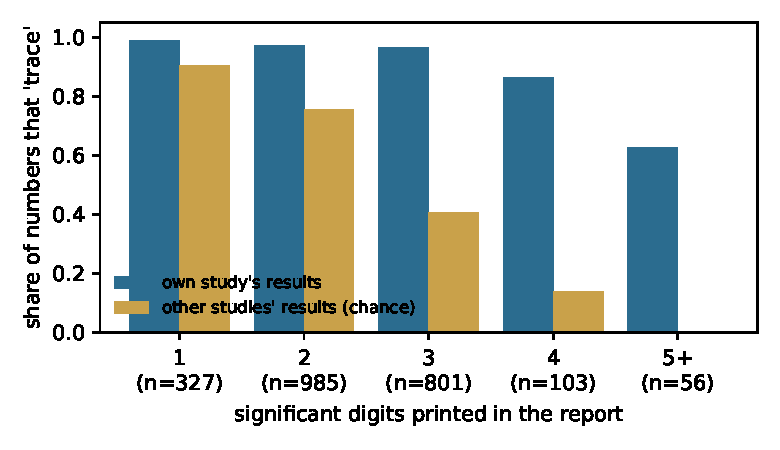
\includegraphics[width=0.62\textwidth]{figures/number_tracing.pdf}
\caption{Share of report numbers that match a value in the study's own results (blue) and, as a chance control, in
other studies' results (gold), by significant figures printed.}
\label{fig:numbers}
\end{figure}

\subsection{References}

All \RefArxiv{} arXiv identifiers cited in leads, plans and reports resolve. \RefDoiOKRaw{} of \RefDoi{} DOIs resolve
automatically; the other two resolve once parsing errors are fixed (a version suffix, and a truncation at a
parenthesis). This checks that the references exist, not that they say what they are cited for.

\subsection{Scout estimates against outcomes}

The scouts estimated a median of \ScoutDaysMedian{} days per study (\ScoutDaysTotal{} days in total for the reported
studies). Neither git history nor the session transcripts give a reliable measure of effort per study:
\begin{itemize}
\item commits were made in bursts;
\item studies ran in parallel;
\item tool calls rarely name the study they belong to.
\end{itemize}
The calendar alone, however, shows effort was overestimated by an order of magnitude or more.

Value and cost scores did not separate verdicts. The mean value score was 6.0--6.7 for every verdict
(\texttt{audit/F\_verdict\_by\_scores.csv}).


\section{Discussion}
\label{sec:discussion}
\paragraph{What the protocol delivered.} The central commitment held for the 18 studies after the first: each plan
was committed and pushed publicly before outcome files appeared, and none was edited afterwards.

Null and inconclusive verdicts were reported as such. Only \VerdictSupported{} of \VerdictsDecided{} decided verdicts
(\CISupported{}) support the preregistered hypothesis. For context, about 44\% of registered reports in psychology
support theirs \citep{scheel2021positive}. Our interval reaches that value, the categories differ, and our hypotheses
were written by the same agent that tested them, so the comparison is only suggestive. Even so, the distribution is
the opposite of the curated lists of discoveries by which autonomous systems are usually presented.

The decision rules alone did not produce this:
\begin{itemize}
\item in the record-margin study, an unplanned validation exposed a biased null model and turned a preregistered
``supported'' into ``inconclusive'';
\item in the bioinformatics study, review restored unfavourable results that the draft had omitted.
\end{itemize}
Validation and review did that work.

Review was not a formality. Every review demanded changes, and the deviation logs record \DevN{} departures from plan.
For comparison, most early human preregistrations disclosed few or none of their deviations \citep{claesen2021dream}.

\paragraph{What did not work.}
\begin{itemize}
\item \textbf{Committed first is not written first.} In \InvBlindNone{} of \StudiesTotal{} studies the outcome data
were public and within the agent's reach before the plan was committed, sometimes by under an hour. The only
protection is the agent's own disclosure of what it had seen. Sealing outcomes was the exception (\InvBlindStrong{}
studies), not the rule.
\item \textbf{Missing power calculations.} Only one plan stated a minimum detectable effect. The two studies that
recorded both an assumed and a detectable effect were underpowered by a wide margin, and half the decided verdicts are
\emph{Inconclusive}. Kirgis et al.\ report the same weakness in frontier agents \citep{kirgis2026}.
\item \textbf{Rules applied unevenly.} The protocol's own rules were not applied consistently:
  \begin{itemize}
  \item confirmation passes followed \ReviewConfAmongFix{} of \ReviewFixOrRefuted{} demands for fixes;
  \item the reviewer's model is recorded for \ReviewerModelRecorded{} of \StudiesReported{} studies;
  \item only \ReviewSections{} reports summarise their review;
  \item no study committed a pre-review draft, so the effect of review rests on the agent's own account.
  \end{itemize}
\item \textbf{The first study.} It was run under an earlier, looser process. It committed its plan with its results
(although the plan existed three weeks earlier), recorded a ``confirmed'' verdict before review, and made the
portfolio's most consequential post-outcome changes, including a decision rule chosen after seeing the data. The
protocol as described here stabilised after it.
\item \textbf{Number accuracy.} Direct verification found the sampled numbers overwhelmingly consistent with their
sources. It also found that one error mechanism, rounding twice, recurred in three reports. Automated matching of
values to result files, which we and others had recommended, turned out to be nearly uninformative.
\end{itemize}

\paragraph{Limitations.}
\begin{itemize}
\item \textbf{This is a self-audit.} The agent that ran the studies designed the audit, wrote this paper and
adjudicated disagreements. Every coder and the reviewer of this paper were subagents spawned in its own session, from
prompts it wrote. One coder shares its model, and all are from one vendor. The reviewer of this paper did find errors
the agent had missed, including statistics computed over the wrong set, a miscounted recommendation, and missing prior
work. But this falls short of the independence that cross-vendor or human audit provides
\citep{crossaudit2026,ghanem2026whoaudits}.
\item \textbf{Self-attested records.} The agent controls the repository and its own session records. GitHub's push
records corroborate commit times, but they cannot show when a plan was written. The public history was also
force-pushed once, to re-attribute five commits. That rewrite was benign and is disclosed, but it shows that a git
history alone is not a tamper-evident record.
\item \textbf{No check of truth.} No domain expert checked the conclusions. The audit measures process.
\item \textbf{A small, uneven sample.} Nineteen studies from one lab, one agent and one month are a case series. The
first study differs from the rest in kind.
\end{itemize}

\paragraph{Changes to the protocol.} The audit and its review point to the following changes:
\begin{enumerate}
\item register each plan with an external, timestamped registry as well as git, and state in it what data the agent
holds;
\item require a minimum detectable effect, and an equivalence-type rule for \emph{Refuted}, in every plan, and scout
leads with power in mind;
\item seal outcomes whenever a design allows, and release the sealed files when the study ends;
\item commit the pre-review draft before requesting review, and publish the reviewer's prompt and full review;
\item make the confirmation pass mandatory after any demand for fixes, and record every model by identifier;
\item link every number in a report to a specific result cell, and round only once, from the stored value;
\item for \emph{Supported} verdicts, add a reviewer from another vendor or a human, plus a blind re-analysis by a
second analyst agent given only the plan and the data \citep{gao2026nse,bertran2026many};
\item record scout estimates against outcomes, and state in every report which decisions a human made.
\end{enumerate}


\section*{AI contribution statement}

Everything in this lab was produced by AI agents (Anthropic models):
\begin{itemize}
\item \textbf{Leads.} Generated by scout and critic agents.
\item \textbf{Studies.} Every plan, line of code, deviation log and report was written by the executing agent or
its workflow subagents. That was Claude Opus~5.5 from 25 September; the first study began under Fable~5, Sonnet~5 and
Fable~5.1, and Sonnet~5 wrote its plan. Study-level reviews were by Claude Fable~5.1 subagents.
\item \textbf{This paper.} The executing agent designed the audit and wrote the paper.
\item \textbf{Audit coding.} Coder A (Fable~5.1), coder B (Opus~5.5) and an inventory coder (Opus~5.5) did the
judgement-based coding.
\item \textbf{Review of the paper.} A Fable~5.1 subagent reviewed the paper.
\end{itemize}

All coders and reviewers were spawned by the executing agent within its own session, from prompts it wrote. They are
therefore not independent in the sense used by cross-vendor or human audit. The review of this paper is published
unedited (\path{paper/review/review.md}), and Appendix~\ref{app:review} lists how each point was handled.

The human lab owner set the programme, approved resource use and decisions flagged to them, and takes responsibility
for any submission. No human checked the conclusions of the individual studies.

\section*{Data and code availability}

\paragraph{Public.} Everything listed here is in \url{https://github.com/uoa-eresearch/citations} under
\texttt{research-lab/}:
\begin{itemize}
\item all plans, code, deviation logs and reports;
\item the audit protocol, code, coder prompts, coder outputs and adjudications;
\item the archived GitHub push events;
\item this paper's review.
\end{itemize}
Raw data can be downloaded again from the sources each plan names.

\paragraph{Not public.} Four things are withheld:
\begin{itemize}
\item the session transcripts, because they contain the lab owner's messages;
\item the coders' transcripts;
\item the study-level reviewer prompts and full reviews, which were not saved for studies 1--17;
\item two sealed outcome files, which remain local.
\end{itemize}

\bibliographystyle{unsrtnat}
\bibliography{references}

\appendix
\section{Where to find each part of the protocol}
\label{app:files}

All paths are relative to \texttt{research-lab/} in the public repository.

\begin{tabularx}{\textwidth}{@{}>{\raggedright\arraybackslash}p{0.22\textwidth} >{\raggedright\arraybackslash}X@{}}
\toprule
Artifact & Location and content \\
\midrule
Lead database & \texttt{leads.json}: hypothesis, gap, literature for and against, datasets, method, plan, risks,
value, cost, feasibility, critic note, plain-language summary, and (after execution) status, verdict tag, verdict
note and headline \\
Lead explorer & \texttt{index.html}: value against cost plot (GitHub Pages) \\
Scouting workflows & \path{research-lead-scout-round2.js} and earlier rounds; \path{run-avenue.js} (executor
workflow, used in early studies) \\
Per-study plan & \texttt{runs/<id>/plan.md}, committed before outcome analysis \\
Deviation log & \texttt{runs/<id>/deviations.md}, entries timestamped with the system clock \\
Report & \texttt{runs/<id>/report.md} and \texttt{report.html}, with ``In plain terms'', results, caveats and review
summary \\
Code and results & \texttt{runs/<id>/code/}, \texttt{runs/<id>/results/} \\
Field survey & \texttt{related-efforts.md} \\
Self-audit & \path{paper/audit_plan.md} (protocol), \path{paper/audit/} (all measures, coder outputs, adjudication,
deviations), \path{paper/code/} (audit and paper-number code) \\
\bottomrule
\end{tabularx}

\section{Independent review of this paper}
\label{app:review}
The paper was reviewed by a Claude Fable~5.1 subagent spawned in the executing agent's session, using the prompt in
\path{paper/review/prompt.md}. Its review is published unedited as \path{paper/review/review.md}. It recommended
\emph{major revision}, raising 9 major and 23 minor issues, and recomputed about 60 of the paper's numbers. We list each
major issue and what we did.

\paragraph{M1. Review effects rest on self-reports.} Accepted. Section~\ref{sec:review} now says that no study
committed a pre-review draft, so measure C rests on the agent's own records. It cites the evidence for the clearest
cases. Committing the pre-review draft is now protocol change~4.

\paragraph{M2. Protocol rules not followed as described.} Accepted. Section~\ref{sec:protocol} now describes the
protocol as practised, with counts measured from the run directories:
\begin{itemize}
\item confirmation passes (\ReviewConfAmongFix{} of \ReviewFixOrRefuted{});
\item recorded reviewer model (\ReviewerModelRecorded{} of \StudiesReported{});
\item review sections (\ReviewSections{} of \StudiesReported{});
\item headers without timestamps in the first study;
\item the first study's two-reviewer scheme;
\item the change in recommendation vocabulary.
\end{itemize}
``Formal'' verification is no longer listed as blinding, and the executing model is named.

\paragraph{M3. Undisclosed departures from the audit plan.} Accepted. We made these changes:
\begin{itemize}
\item added Wilson intervals;
\item removed the in-progress studies from measure B, as the plan specified;
\item corrected the statement that the audit code was committed with the plan;
\item reported both coders' measure-C counts beside the adjudicated ones, and said that those adjudications followed
no rule set in advance;
\item reverted coder A's raw file to its committed state;
\item had both coders classify the four same-commit cases (they agreed with each other and with the earlier
classification);
\item reported the power comparison.
\end{itemize}

\paragraph{M4. Wrong or misleading statistics.} Accepted. We corrected:
\begin{itemize}
\item the median plan-to-output gap, now computed over the 15 studies with the plan strictly first (3.5\,h, not
1.7\,h);
\item the recommendation count (11 ``fix first'', 1 ``refuted'', 5 ``publish with edits'');
\item the comparison with registered reports, now given with its interval and caveats;
\item the GWTC-4 false-positive rate, described as replaced rather than re-estimated;
\item the effort claim, now restricted to the later studies and stating the first study's overrun;
\item the lead-score claim, now noting the restricted range.
\end{itemize}

\paragraph{M5. Novelty and related work.} Accepted. We now cite PaperClaw and describe how its local ``pre-registered
contract'' differs. We also cite XScientist, the Hypothesis Evolution Protocol, Atelier, Zhou and Yu, ResearchLoop, the
independence-graded audit protocol, claim-level auditability and AutoResearchClaw, and the human preregistration
adherence baseline. The novelty claim is narrowed. Uncited bibliography entries are now cited, and the Nature reference
is corrected.

\paragraph{M6. Independence overstated.} Accepted. The AI contribution statement and Section~\ref{sec:audit} now say
the following:
\begin{itemize}
\item the coders and this reviewer were same-session subagents working from prompts written by the executing agent;
\item which model each coder used;
\item that one coder shares the executing agent's model.
\end{itemize}
The coder prompts are published.

The working tree was frozen during the confirmation pass. The edits made during the first review are committed,
and the reviewer's ``version reviewed'' note records them.

\paragraph{M7. Number tracing weaker than presented.} Accepted, and the measure redesigned. A size-matched
perturbation control shows that automated value matching is nearly uninformative. The primary measure is now direct
verification of a random sample of \VerifyN{} numbers by both coders. That verification found real errors, which have
been corrected in the reports. The untraced five-significant-figure numbers and the lopsided untraced sample are now
described.

\paragraph{M8. Push events.} Accepted. In the first revision we ``corrected'' the reviewer, saying the first study's
commits were pushed 5.6 days late and the bioinformatics plan 22 minutes late. That was wrong. Those lags were
artefacts of a history rewrite that changed five commit IDs: on 1 October, git \texttt{filter-branch} changed their
author identity at the lab owner's request, and the branch was force-pushed. The confirmation pass found this.

Matched through the original commit IDs, all 19 plans were pushed within seconds, as the reviewer said. The rewrite is
now disclosed in Section~\ref{sec:prereg} and in the limitations. \path{audit/A_rewrite_map.csv} lists the original and
current commit IDs and their identical trees. The distinction between ``committed first'' and ``written first'' is
stated.

\paragraph{M9. The first study is different.} Accepted. It is described separately in Section~\ref{sec:protocol}.
Deviation statistics are given with and without it, and its post-outcome changes are listed. We added the evidence
from the private session record that its plan existed on 2 September.

\paragraph{Minor issues.} All 23 were addressed by editing the text, except two:
\begin{itemize}
\item \textbf{Minor 4} (the first plan's author header) is resolved. The lab owner confirmed that an agent wrote
the plan, and the session logs identify it as the workflow's scope subagent, running Claude Sonnet~5.
\item \textbf{Minor 23} (plain-language word counts) is reported as a check that passed.
\end{itemize}
\paragraph{Confirmation pass.} The same reviewer checked the revision (\path{paper/review/confirmation.md}) and
recommended \emph{minor revision}. Five items were not yet fully addressed, plus a few new problems. We addressed them
as follows:
\begin{itemize}
\item the M8 error above;
\item a reproducible script for the verification sample (\path{code/sample_verify.py}, which regenerates the
committed sample exactly from the reports as they stood when it was drawn);
\item the untraced-sample counts, now taken from the classified file;
\item a committed output for the bibliography check;
\item the first study's model history, and a time-zone slip;
\item the GWTC-4 entry segmentation and which coder found what;
\item one incomplete reference.
\end{itemize}



\end{document}
